\begin{figure*}[tp]
\centering
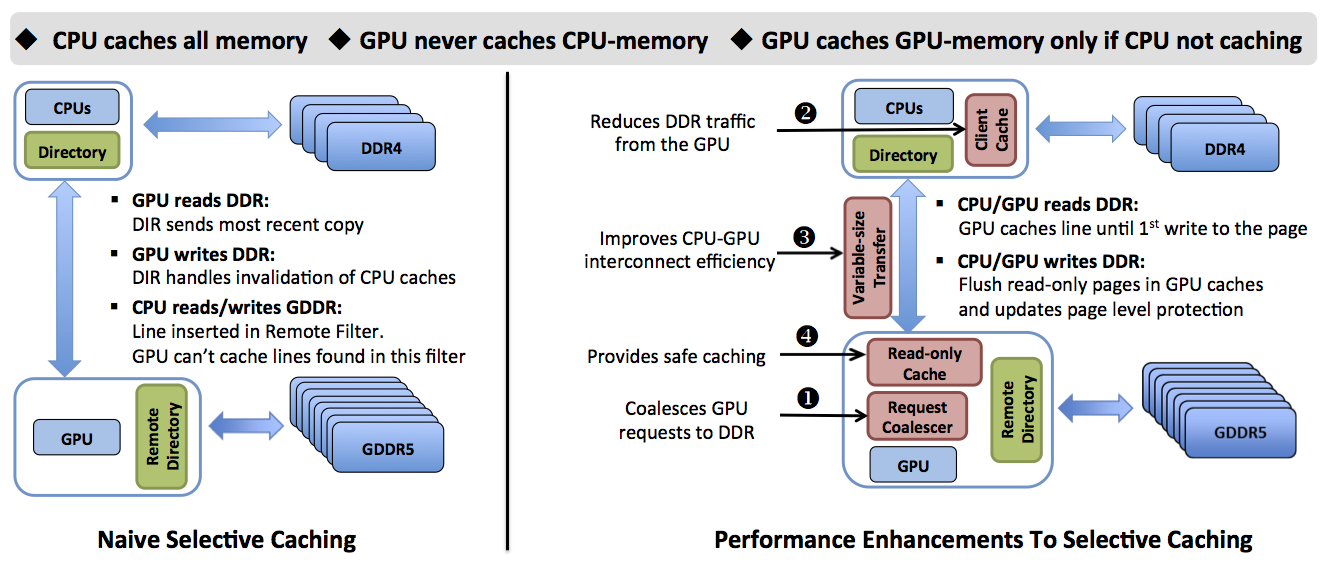
\includegraphics[width=0.9\textwidth]{figures/coherence_overview.png}
\caption{Overview of naive selective caching implementation and optional performance enhancements.
Selective caching GPUs maintain memory coherence with the CPU while not
requiring hardware cache coherence within the GPU domain.}
\label{fig:coherence_overview}
% \vspace{.05in}
\end{figure*}

\section{GPU Selective Caching}
\label{proposal}

Historically, GPUs have not required hardware cache coherence because their
programming model did not provide a coherent address space between threads running on separate
SMs~\cite{CUDA7}.  CPUs however, support hardware cache coherence 
because it is heavily relied upon by both system and application
programmers to ensure correctness in multi-threaded programs. 
Existing GPU programming models do not guarantee data correctness when CPU and GPU accesses
interleave on the same memory location while the GPU is executing. One way to
provide such guarantees is to enforce CPU--GPU hardware cache coherence, albeit with significant implementation 
complexity as previously discussed.

Alternatively, if the GPU does not cache any data that is concurrently cached by the CPU,
no hardware coherence messages need to be exchanged between the CPU and GPU, yet data correctness is still guaranteed. 
This approach also decouples
the, now private, coherence protocol decisions in CPU and GPU partitions, facilitating multi-vendor 
system integration.  We now discuss how CPU--GPU
memory can provide this single shared memory abstraction without implementing 
hardware cache coherence. We then propose several micro-architectural enhancements to enable selective caching
to perform nearly as well as hardware cache coherence, while maintaining the programmability benefits of hardware cache coherence.

\subsection{Naive Selective Caching}
\label{naiveselectivecaching}

As shown in Figure~\ref{fig:coherence_overview},
three simple principles enable the GPU to support a CPU-visible shared memory
by implementing selective caching. First, the CPU is always allowed to cache any data in the system regardless 
of whether that data is physically located in the memory attached to the GPU or the CPU\@. 
Second, the GPU is never allowed to cache data that resides within the 
CPU memory.  Finally, the GPU may cache data from its 
own local memory if and only if the CPU is not also caching a copy of this 
data.

When the CPU is known to be caching a line that is homed in GPU memory and the GPU requests
this line, the request must be routed to the CPU where the requested data is serviced 
from the CPU cache, rather than the GPU memory. Similarly, if the GPU is caching a 
line that the CPU requests, then this line must be flushed from the GPU caches when the 
request is received by the GPU memory controller. By dis-allowing caching 
of memory in use by the CPU, the GPU cannot violate the CPU hardware coherence model.

The primary microarchitectural structure needed by the GPU to implement
selective caching is the \emph{remote directory}. The remote directory block
shown in Figure~\ref{fig:coherence_overview} tracks approximately, but conservatively,
the cache lines homed in GPU  memory that are presently cached at the CPU.
When the CPU requests a line from GPU memory,  its cache block address is  
entered into the remote directory.  If the address was not already present, the GPU
probes and discards the line from all GPU caches, as in a conventional invalidation-based 
coherence protocol.  Once a cache block is added to the GPU remote
directory, it becomes un-cacheable within the GPU; future GPU accesses to the line
will be serviced from the CPU cache.

To limit hardware cost, we implement the remote directory as a cuckoo filter 
(a space efficient version of a counting bloom filter) that never reports
false negatives but may report false positives~\cite{fan2014,bonomi2006}. Thus, the remote directory may erroneously, but conservatively,
indicate that a line is cached at the CPU that has never been requested, but will accurately reference
all lines that have actually been requested.  False positives in the remote directory generate
a spurious request to the CPU, which must respond with a negative acknowledgement (NACK) should the line
not be present in the CPU cache.  This request will then be serviced from the GPU memory
system.  Similarly, if the CPU has cached a line homed in GPU memory (causing a remote directory insertion)
and has since evicted it, the CPU may also NACK a GPU request, causing the request to return to the GPU memory
for fulfillment.

Because entries are inserted but never pruned from our remote directory, we must track if the directory
becomes full or reaches a pre-selected high-water mark.  If it becomes full, our implementation
forces the CPU to flush all cache lines homed in GPU memory and then resets the remote directory.  This limited
cache flush operation  does not flush any lines
homed in CPU memory, the vast majority of the system's memory capacity.  In our
design, the flush is performed by triggering a software daemon to call the Linux \texttt{cacheflush} trap.  

The remote directory is sized to track CPU caching of up to 8MB of GPU memory, which when fully occupied
requires just 64KB of on-chip storage to achieve a false positive rate of 3\%.  In the workloads we evaluate,
the remote directory remains largely empty, and neither the capacity nor false positive rate have a significant
impact on GPU performance.
If workloads emerge that 
heavily utilize concurrent CPU--GPU threads, the size and performance of this structure will need to be re-evaluated. 
However if \texttt{cacheflush} trapping should become excessive due to an undersized remote directory,
page-migration of CPU--GPU shared pages out of GPU memory and into CPU memory can also be employed to 
reduce pressure on the GPU remote directory.

\subsection{Improving Selective Caching Performance}
\label{microarchimprovements}

Caches have consistently been shown to provide significant performance 
gains thanks to improved bandwidth and latency.  As such, naively bypassing the GPU caches based on the mechanisms described in 
Section~\ref{naiveselectivecaching} should be expected to hurt performance. In this subsection, we describe 
three architectural improvements that mitigate the impact of selectively bypassing the GPU caches and provide performance approaching
a system with hardware cache coherence.

\subsubsection{Cacheless Request Coalescing}
\label{coalescing}

The first optimization we make to our naive
selective caching design is to implement aggressive miss status handling register (MSHR)
request coalescing for requests sent to CPU memory, labeled \mycirc{1} in Figure~\ref{fig:coherence_overview}.  
MSHR request coalescing can significantly reduce the request traffic
to CPU memory without violating coherency guarantees.
Request coalescing works by promoting
the granularity of an individual load request (that may be as small as 64 bits)
to a larger granularity (typically 128B cache lines) before issuing the request
to the memory system.  While this larger request is in-flight, if other requests
are made within the same 128B block, then these requests
can simply be attached to the pending request list in the corresponding MSHR and no new request is issued
to the memory system.

To maintain correctness in a selective caching system, this same coalescing
scheme can be utilized, but data that is returned to the coalesced requests for which no pending
request is found must be discarded immediately. Discarding data in this way is similar to self-invalidating
coherence protocols, which attempt to minimize invalidation traffic in CC-NUMA
systems~\cite{Lebeck95,Lai2000}.  Whereas most MSHR implementations allocate their storage in
the cache into which the pending request will be inserted, our cache-less request coalescing must have
local storage to latch the returned data.  This storage overhead is negligible compared to the aggregate
size of the on-chip caches that are no longer needed with selective caching.

Table~\ref{tab:coalescing_opportunity} shows the fraction of GPU memory requests 
that can be coalesced by matching them to pre-existing in-flight memory requests.
We call request coalescing that happens within a single 
SM \emph{L1 coalescing} and coalescing across SMs \emph{L1+L2 coalescing}.  
On average, 35\% of memory requests can be serviced via 
cacheless request coalescing.  While a 35\% hit rate may seem low when
compared to conventional CPU caches, we observe that capturing spatial request locality
via request coalescing provides the majority of the benefit of the L1 caches (44.4\% hit rate) found
in a hardware cache-coherent GPU, as shown in Table~\ref{tab:gpuhitrate}.

\begin{table}[tp]
\begin{center}
\begin{tabular}{ddd}
 \hline
 \multicolumn{1}{l}{Workload}  &  \multicolumn{1}{c}{L1 Coalescing}  &  \multicolumn{1}{c}{L1+L2 Coalescing}  \\
 \hline
 \hline
 \multicolumn{1}{l}{backprop}  &   54.2  &   60.0   \\
 \hline
 \multicolumn{1}{l}{bfs}  &   15.8  &   17.6   \\
 \hline
 \multicolumn{1}{l}{btree}  &   69.4  &   82.4   \\
 \hline
 \multicolumn{1}{l}{cns}  &   24.8  &   28.1   \\
 \hline
 \multicolumn{1}{l}{comd}  &   45.7  &   53.8   \\
 \hline
 \multicolumn{1}{l}{kmeans}  &   0.0  &   0.0   \\
 \hline
 \multicolumn{1}{l}{minife}  &   29.0  &   32.6   \\
 \hline
 \multicolumn{1}{l}{mummer}  &   41.9  &   51.1   \\
 \hline
 \multicolumn{1}{l}{needle}  &   0.1  &   1.8   \\
 \hline
 \multicolumn{1}{l}{pathfinder}  &   41.4  &   45.8   \\
 \hline
 \multicolumn{1}{l}{srad\_v1}  &   30.8   &   34.2   \\
 \hline
 \multicolumn{1}{l}{xsbench}  &   15.6  &   18.0   \\
 \hline
 \hline
 \multicolumn{1}{l}{Average}  &   30.7  &   35.4  \\
\hline
\end{tabular}
\caption{Percentage of memory accesses that can be coalesced into existing 
in-flight  memory requests, when using L1 (intra-SM) coalescing, and L1 + L2 (inter-SM) 
coalescing.}
\label{tab:coalescing_opportunity}
\end{center}
\vspace{-.1in}
\end{table}

\subsubsection{CPU-side Client Cache}
\label{clientcache}

Although memory request coalescing provides hit rates approaching that of
conventional GPU L1 caches, it still falls short as it cannot capture
temporal locality. Selective caching prohibits the GPU from locally caching lines 
that are potentially shared with the CPU but it does not preclude the GPU from remotely 
accessing coherent CPU caches.
We exploit this opportunity to propose a \textit{CPU-side GPU client cache}  (label \mycirc{2} in Figure~\ref{fig:coherence_overview}), which takes 
advantage of temporal locality not exploited by MSHR coalescing.

To access CPU memory, the GPU must already send a request to the CPU
memory controller to access the line. If request coalescing has failed to
capture re-use of a cache line, then multiple requests for the same line will
be sent to the CPU memory controller causing superfluous transfers across the DRAM
pins, wasting precious bandwidth.  To reduce this DRAM pressure, we introduce a small 
client cache at the CPU memory controller to service
these GPU requests, thereby shielding the DDR memory system from
repeated requests for the same line.  Our proposed GPU client cache participates in the 
CPU coherence protocol much like any other 
coherent cache on the CPU die, however lines are allocated in this cache only upon 
request by an off-chip processor, such as the GPU\@.

This single new cache does not introduce the 
coherence and interconnect scaling challenges of GPU-side caches,
but still provides some latency and bandwidth filtering advantages
for GPU accesses. One might consider an alternative where GPU-requested lines are instead injected into
the existing last-level cache (LLC) at the CPU.  In contrast to an injection approach, our
dedicated client cache avoids thrashing the CPU LLC 
when the GPU streams data from CPU memory (a common access pattern).
By placing this client cache on the CPU-side rather than the GPU-side of the CPU--GPU 
interconnect, we decouple the need to extend the CPU's hardware cache coherence protocol into even one on-die GPU cache.
However, because the GPU client cache is located at the CPU-side of the CPU--GPU interconnect,
it provides less bandwidth than a GPU-side on-die cache. As described in Section~\ref{background} and 
shown in Figure~\ref{fig:cache_bw_latency}, this bandwidth loss is typically not performance-critical.

\subsubsection{Variable-size Link Transfers}
\label{variablesizing}

Conventional memory systems access data at cache line granularity to 
simplify addressing and request matching logic, improve DRAM energy consumption, and 
exploit spatial locality within caches.  Indeed, the minimum transfer size supported
by DRAM is usually a cache line.  Cache line-sized transfers work well when data
that was not immediately needed can be inserted into an on-chip cache, but
with selective caching, unrequested data transferred from CPU memory must be discarded.  
Hence, portions of a cache line that
were transferred, but not matched to any coalesced access, result in wasted
bandwidth and energy. 

The effect of this data over-fetch is shown in
Table~\ref{tab:overfetch}, where cache line utilization is the fraction of the transferred
line that has a pending request when the GPU receives a cache line-sized response from CPU  memory.
An average cache line utilization of 60\% indicates that just 77 out of 128 bytes transferred are actually used by
the GPU\@. 51 additional bytes were transferred across the DRAM interface and CPU--GPU interconnect 
only to be immediately discarded.

\begin{table}[tp]
\begin{center}
\begin{tabular}{dd}
 \hline
 \multicolumn{1}{l}{Workload}  &  \multicolumn{1}{c}{Avg. Cacheline Utilization(\%)}  \\
 \hline
 \hline
 \multicolumn{1}{l}{backprop}  &   85.9  \\
 \hline
 \multicolumn{1}{l}{bfs}  &   37.4  \\
 \hline
 \multicolumn{1}{l}{btree}  &   78.7  \\
 \hline
 \multicolumn{1}{l}{cns}  &   77.6  \\
 \hline
 \multicolumn{1}{l}{comd}  &   32.6  \\
 \hline
 \multicolumn{1}{l}{kmeans}  &   25.0  \\
 \hline
 \multicolumn{1}{l}{minife}  &   91.6  \\
 \hline
 \multicolumn{1}{l}{mummer}  &   46.0  \\
 \hline
 \multicolumn{1}{l}{needle}  &   39.3  \\
 \hline
 \multicolumn{1}{l}{pathfinder}  &   86.6  \\
 \hline
 \multicolumn{1}{l}{srad\_v1}  &   96.3  \\
 \hline
 \multicolumn{1}{l}{xsbench}  &   30.3  \\
 \hline
 \hline
 \multicolumn{1}{l}{Average}  &   60.6  \\
\hline
\end{tabular}
\caption{Utilization of 128B cache line requests where the returned data 
must be discarded if there is no matching coalesced request.}
\label{tab:overfetch}
\end{center}
\vspace{-.1in}
\end{table}

To address this inefficiency, architects might consider reducing the
transfer unit for selective caching clients from 128B down to 64 or 32 bytes. While 
fine-grained transfers improve transfer efficiency by omitting unrequested data, that
efficiency is offset by the need for multiple small requests and packetization
overhead on the interconnect. For example, in our link implementation,
a transfer granularity of 32B achieves at best 66\% link utilization (assuming
all data is used) due to interconnect protocol overheads, while
128B transfers (again, assuming all data is used) can achieve 88\% efficiency.

To maintain the benefit of request coalescing, but reduce interconnect
inefficiency, we propose using \textit{variable-size transfer units} on the 
CPU--GPU interconnect (labeled \mycirc{3} in Figure~\ref{fig:coherence_overview}).  
To implement variable-size transfer units at the GPU, we allocate GPU MSHR entries at the full
128B granularity; coalescing requests as described in Section~\ref{coalescing}.  However, 
when a request is issued across the CPU--GPU interconnect, we embed a bitmask in the 
request header indicating which 32B sub-blocks of the 128B cache line should be transferred on the return path.
While this initial request is pending across the interconnect, if additional requests
for the same 128B cache line are made by the GPU, those requests will be issued across the interconnect
and their 32B sub-block mask will be merged in the GPU MSHR.  

Similar to the GPU-side MSHR, variable sized transfer units require that the CPU-side client cache also maintain pending MSHR
masks for requests it receives, if it can not service the requests immediately from the
cache.  By maintaining this mask, when the DRAM returns the 128B line, only those
32B blocks that have been requested are transferred to the GPU (again with a bitmask indicating
which blocks are included).  Because there may be
both requests and responses in-flight simultaneously for a single 128B line, it is possible
that two or more responses are required to fulfill the data requested by a single MSHR; the bitmasks
included in each response facilitate this matching.
Because GPUs typically perform SIMD lane-level request coalescing within an SM, 32B requests happen 
to be the minimum and most frequently sized request issued to the GPU memory system.  As a result, we do 
not investigate supporting link transfer sizes smaller than 32 bytes, which would require microarchitectural
changes within the GPU SM.

\subsection{Promiscuous Read-Only Caching}
\label{readonly}

Selective caching supports coherence guarantees by bypassing GPU caches when
hardware cache-coherence operations could be needed.  Thus far, our selective caching architecture
has assumed that the GPU must avoid caching all data homed in CPU memory.  We identify
that we can loosen this restriction and allow GPU caching of CPU memory, but only
if that data can be guaranteed to be read-only by both the CPU and GPU.

Figure~\ref{fig:readonlymotivation} shows the fraction of data touched by the 
GPU that is read-only or both read and written, broken down at 
the OS page (4KB) granularity.  In many workloads, we find the majority 
of the data touched by the GPU is read-only at the OS page level.  We
examine this data at page granularity because, even without hardware 
cache coherence, it is possible (though expensive) to\ignore{ implement coherence}
guarantee correctness through OS page 
protection mechanisms entirely in software. 
Any cache may safely contain data from read-only OS pages.
However, if the page is re-mapped as read-write, cached copies
of the data at the GPU must be discarded, which will occur as part
of the TLB shootdown process triggered by the permission change~\cite{stenstrom1990}.

\begin{figure}[tp]
\centering
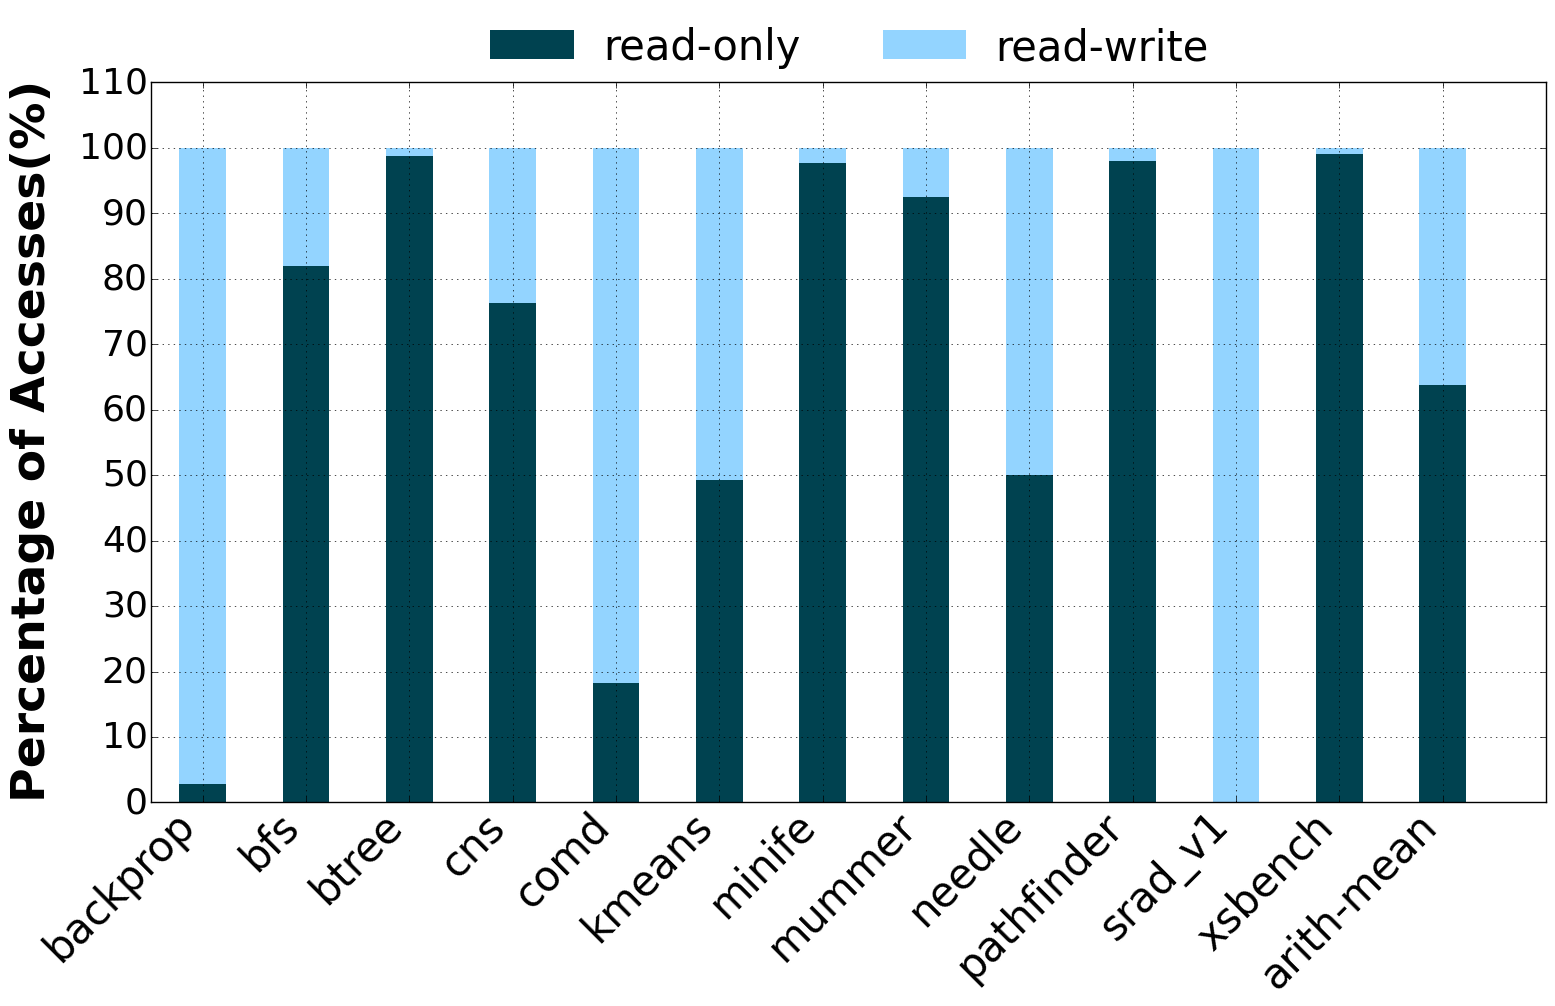
\includegraphics[width=1.0\columnwidth]{figures/read-only.png}
\caption{Fraction of 4KB OS pages that are read-only and read-write
during GPU kernel execution.}
\label{fig:readonlymotivation}
% \vspace{-.1in}
\end{figure}

We propose that despite lacking hardware cache coherence, selective caching GPUs may choose to implement 
\textit{promiscuous read-only caching of CPU-memory}, relying on such page level software coherence 
to provide correctness (labeled \mycirc{4} in Figure~\ref{fig:coherence_overview}).  To implement read-only caching, the GPU software 
run-time system speculatively marks pages within the application as 
read-only at GPU kernel launch time.  It also tracks which pages may have been marked
read-only by the application itself to prevent speculation conflicts.  With pages speculatively
marked as read-only, when the GPU requests pages from the CPU memory, the permissions 
bit in the TLB entry is checked to determine if lines from this page are cacheable by the 
GPU\@ despite being homed in CPU memory. Similarly, if the line resides in GPU memory but is marked as cached by
the CPU in the remote directory, this line can still be cached locally because it is read-only.

If a write to a read-only page occurs at either the CPU or GPU, a protection
fault is triggered. A write by the CPU invokes a fault handler
on the faulting core, which marks the line as read/write at the CPU and
uncacheable at the GPU.  The fault handler then triggers a TLB shootdown,
discarding the now stale TLB entry from all CPU and GPU TLBs.
This protection fault typically incurs a 3-5us delay.  The next access
to this page at a GPU SM will incur a hardware page walk to refetch this PTE, 
typically adding < 1us to the first access to this updated page.

A faulting write at the GPU is somewhat more complex, as protection fault
handlers currently do not run on a GPU SM.  Instead, the GPU MMU must
dispatch an interrupt to the CPU to invoke the fault handler.  That SW handler
then adjusts the permissions and shoots down stale TLB entries, including those at the GPU.
The CPU interrupt overhead raises the total unloaded latency of the fault to ~20us (as measured
on NVIDIA's Maxwell generation GPUs). However, only the faulting warp is stalled: the SM can
continue executing other non-faulting warps.  Once the GPU receives an acknowledgement that the
fault handling is complete, it will re-execute the write, incurring a TLB miss
and a hardware page walk to fetch the updated PTE entry.

The many-threaded nature of the GPU allows us to largely hide 
the latency of these permission faults by executing other warps, thereby mitigating 
the performance impact of the high SW fault latency in nearly all of our workloads.
Nevertheless, software page fault handlers are orders of magnitude more expensive
than hardware cache-coherence messaging and may erode the benefit of promiscuous 
read-only caching if permission faults are frequent.  We evaluate the performance of promiscuous 
caching under different software faulting overhead costs in Section~\ref{readonlyresults}.
